\section{Evaluation}\label{evaluation}
This section reveals the evaluation of SCache with comprehensive workloads and benchmarks. 
First we run a job with single shuffle to analyze hardware utilization and see the impacts of different components from the scope of a task to a job. 
Then we use a recognized shuffle intensive benchmark --- Terasort to evaluate SCache with different data partition schemes.

\begin{figure}
	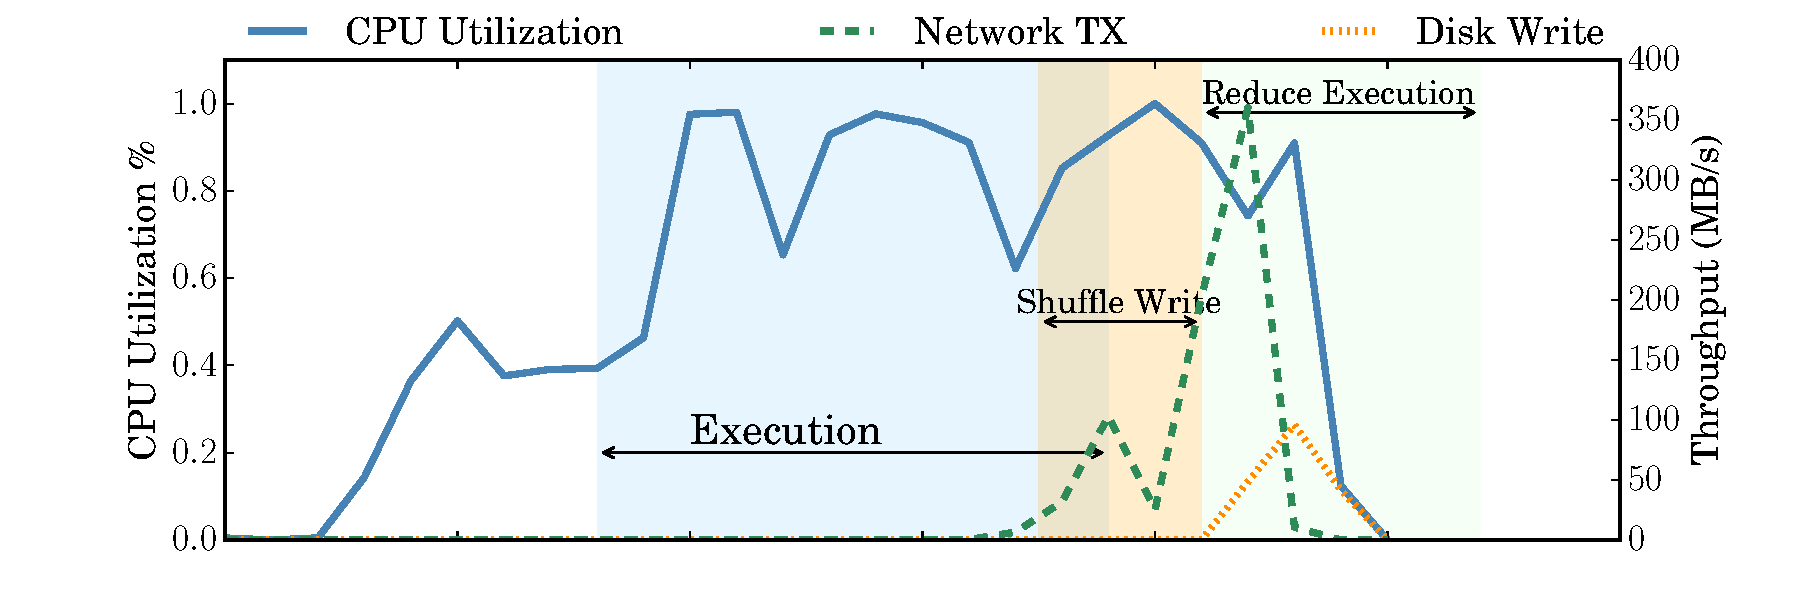
\includegraphics[width=\linewidth]{fig/scache_util}
	\caption{CPU utilization and I/O throughput of a node during a Spark single shuffle application With SCache}
	\label{fig:scache_util}
\end{figure}

In order to prove the performance gain of SCache with a real production workload, we also evaluate Spark TPC-DS\footnote{https://github.com/databricks/spark-sql-perf} and present the overall performance improvement.
{\color{blue}
To prove SCache compatibility as a cross-framework plug-in, we implemented SCache on both Hadoop MapReduce and Spark. 
Due to the simple DAG computing in Hadoop MapReduce, we only use Terasort as a shuffle-heavy benchmark to evaluate the performance of Hadoop MapReduce with SCache.
}
Finally, we measure the overhead of weighted reservoir sampling. 
In summary, SCache can decrease ~$89\%$ time of Spark shuffle without introducing extra network transfer.
More impressively, the overall completion time of TPC-DS can be improved ~$40\%$ on average by applying the optimization from SCache.
{\color{blue}Meanwhile, Hadoop MapReduce with SCache optimize job completion time by up to 15\% and an average of 13\%}

% Because a complex Spark application consists of multiple stages. The completion time of each stage varies under different input data, configurations and different number of stages. This uncertainty leads to the dilemma that dramatic fluctuation occurs in overall performance comparison. To present a straightforward illustration, we limit the scope of most evaluations in a single stage.
\begin{figure*}
	\centering
	\begin{minipage}[t]{.32\linewidth}
		\begin{subfigure}{\linewidth}
			\begin{minipage}{\linewidth}
				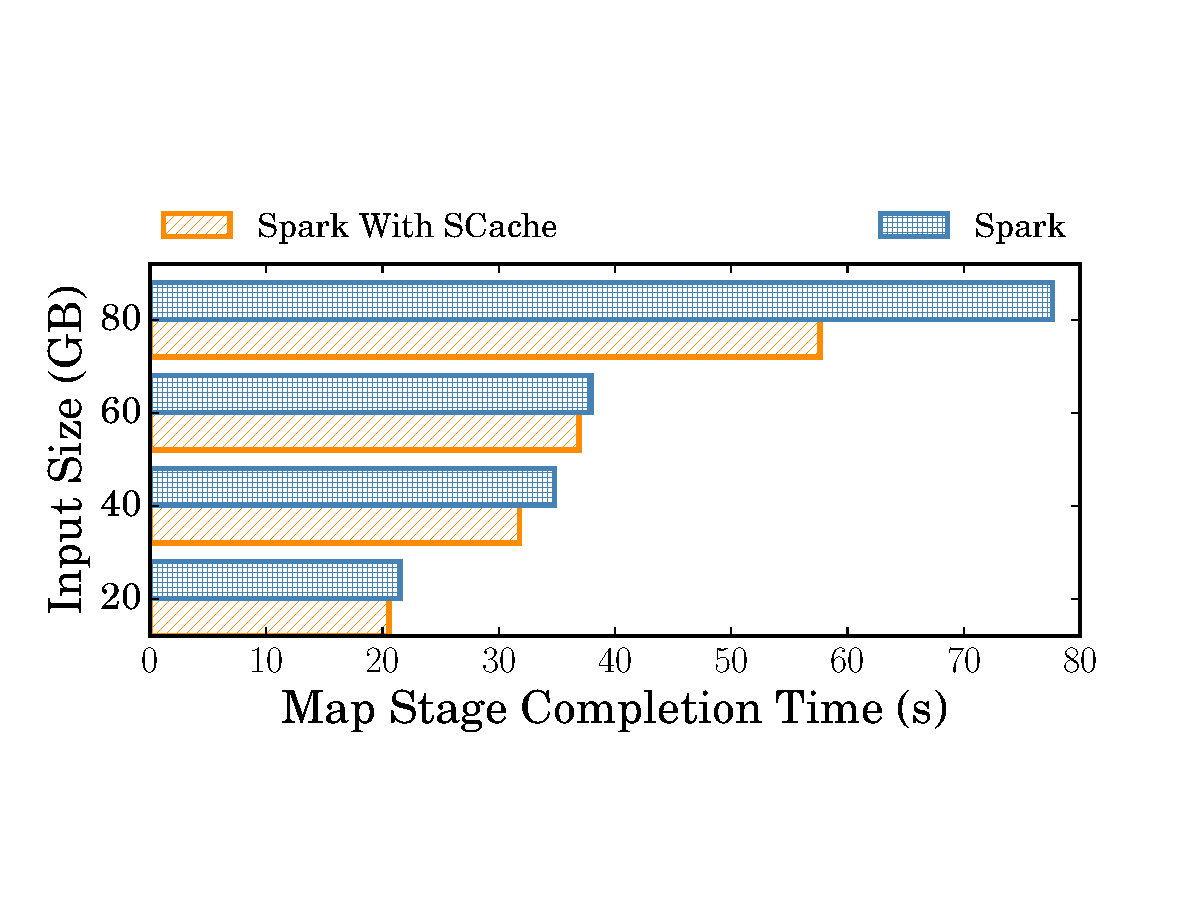
\includegraphics[width=\linewidth]{fig/groupbymapstage}
				\caption{Map Stage Completion Time}
				\label{fig:mapstage}
			\end{minipage}
			\begin{minipage}{\linewidth}
				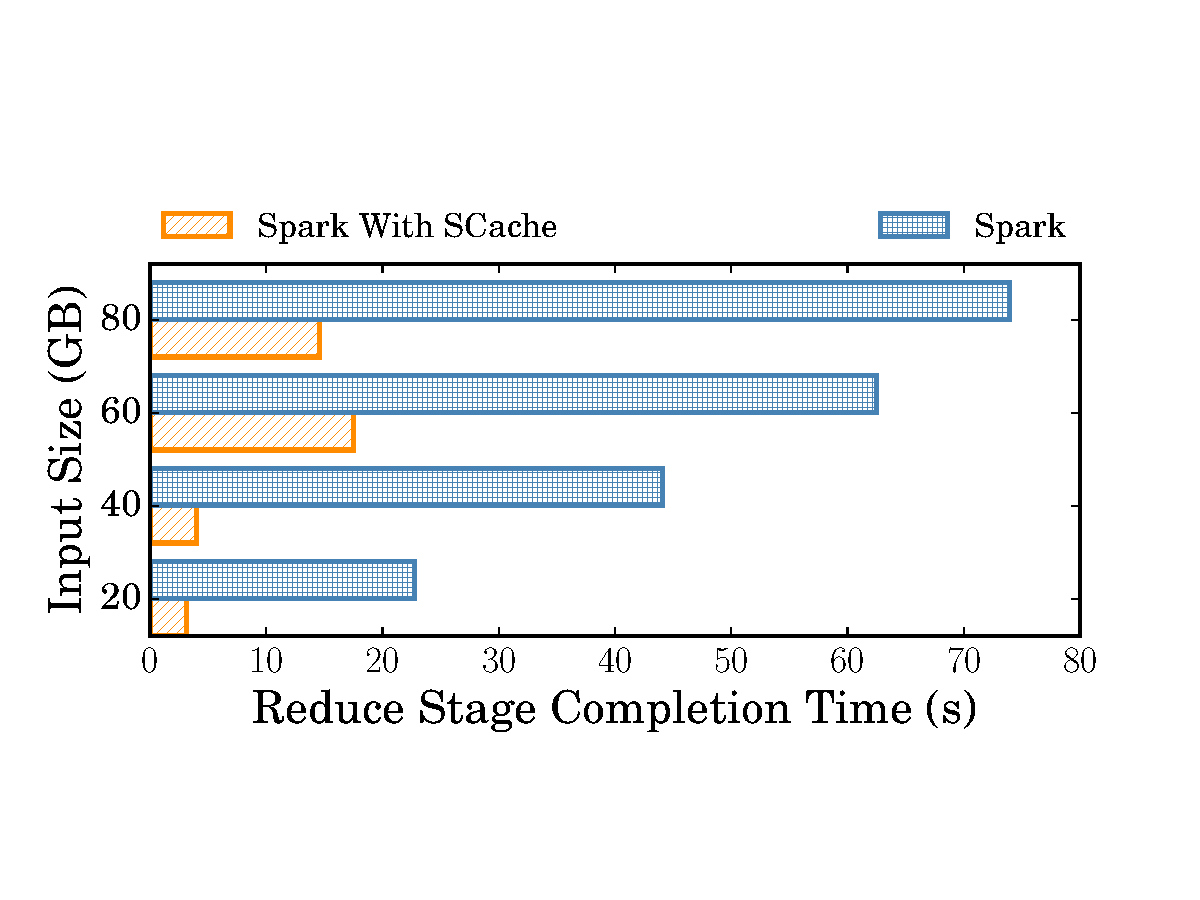
\includegraphics[width=\linewidth]{fig/groupbyreducestage}
				\caption{Reduce Stage Completion Time}
				\label{fig:reducestage}	
			\end{minipage}
		\end{subfigure}
		\caption{Stage Completion Time of Single Shuffle Test}
		\label{fig:singleshuffle}
	\end{minipage}	
	\begin{minipage}[t]{.32\linewidth}
		\begin{subfigure}{\linewidth}
			\begin{minipage}{\linewidth}
				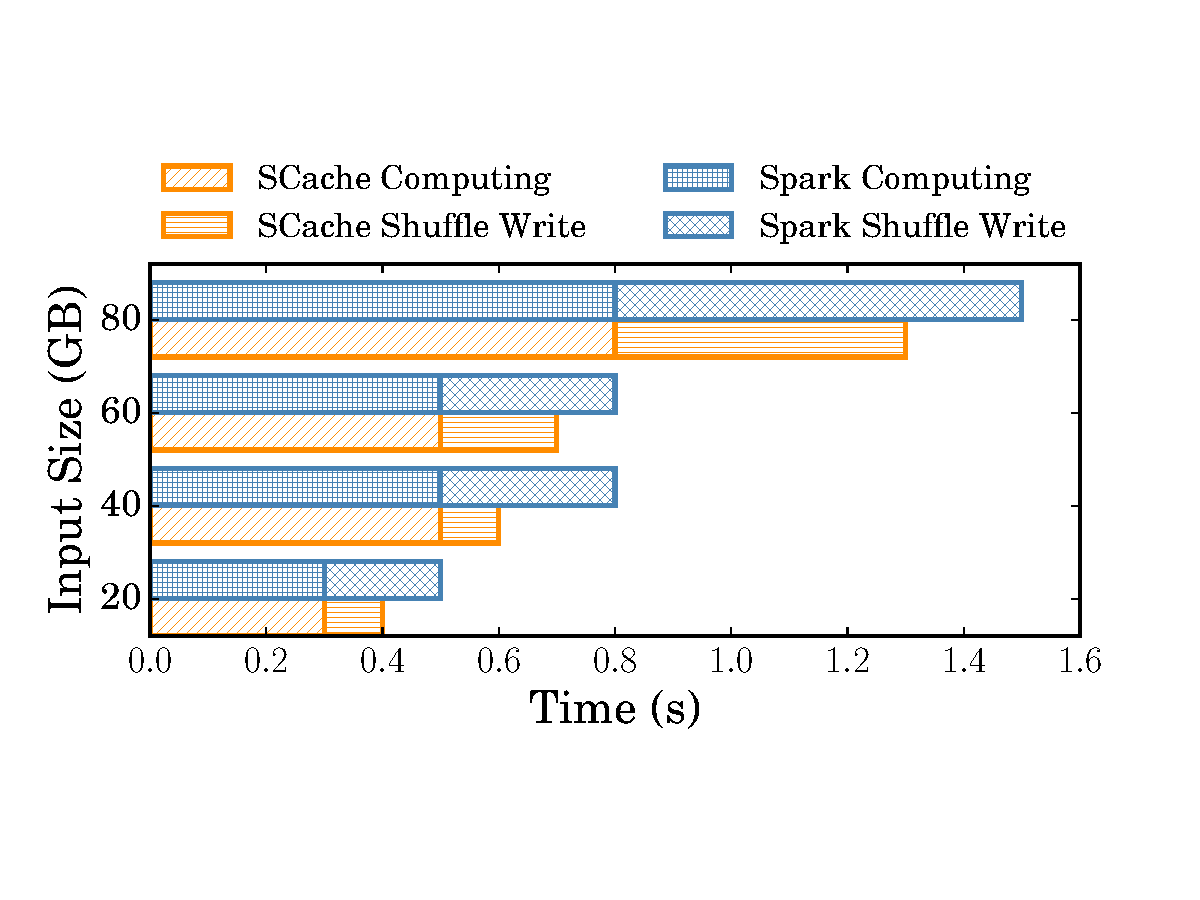
\includegraphics[width=\linewidth]{fig/groupbymaptask}
				\caption{Median Task in Map Stages}
				\label{fig:maptask}
			\end{minipage}

			\begin{minipage}{\linewidth}
				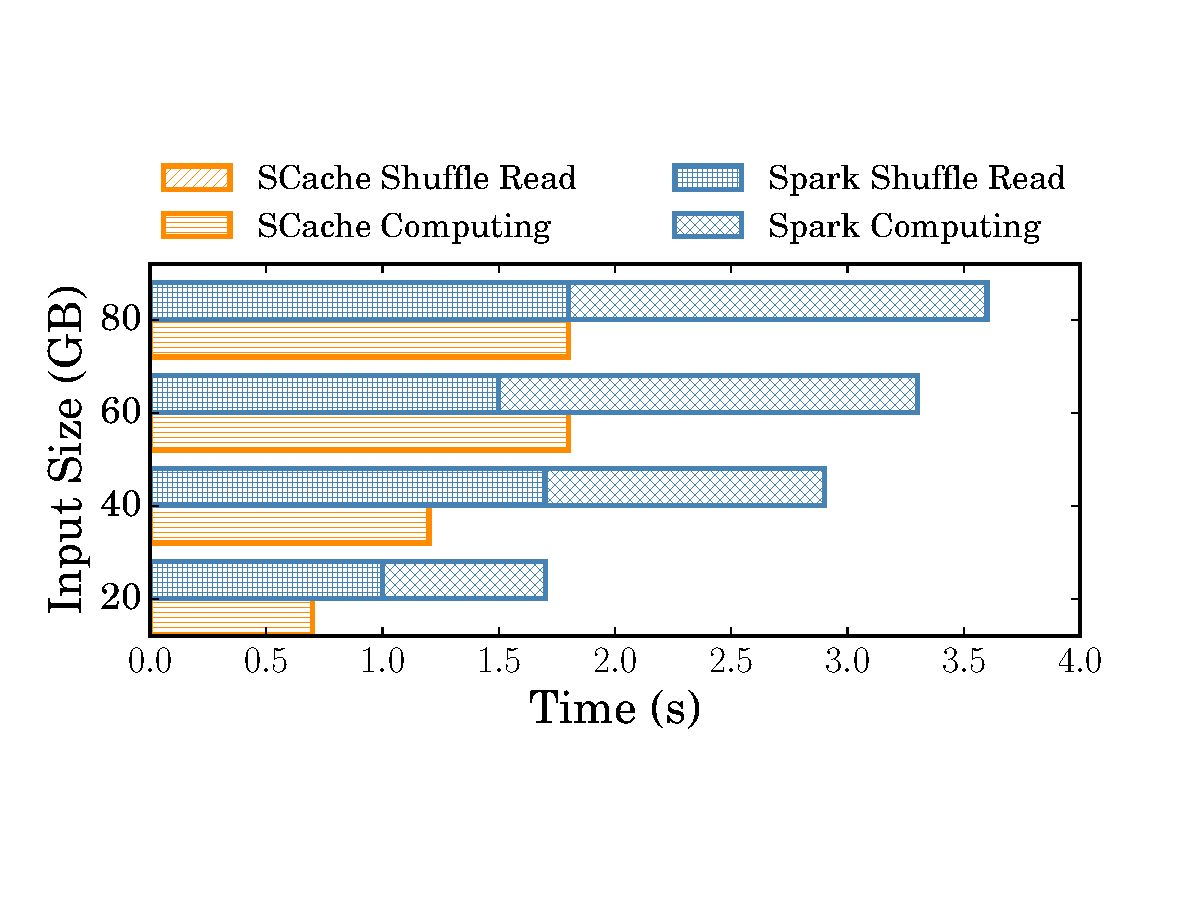
\includegraphics[width=\linewidth]{fig/groupbyreducetask}
				\caption{Median Task in Reduce Stages}
				\label{fig:reducetask}
			\end{minipage}
		\end{subfigure}
		\caption{Median Task Completion Time of Single Shuffle Test}
		\label{fig:singleshuffletask}
	\end{minipage}	
	\begin{minipage}[t]{.32\linewidth}
		\begin{subfigure}{\linewidth}
			\begin{minipage}{\linewidth}
				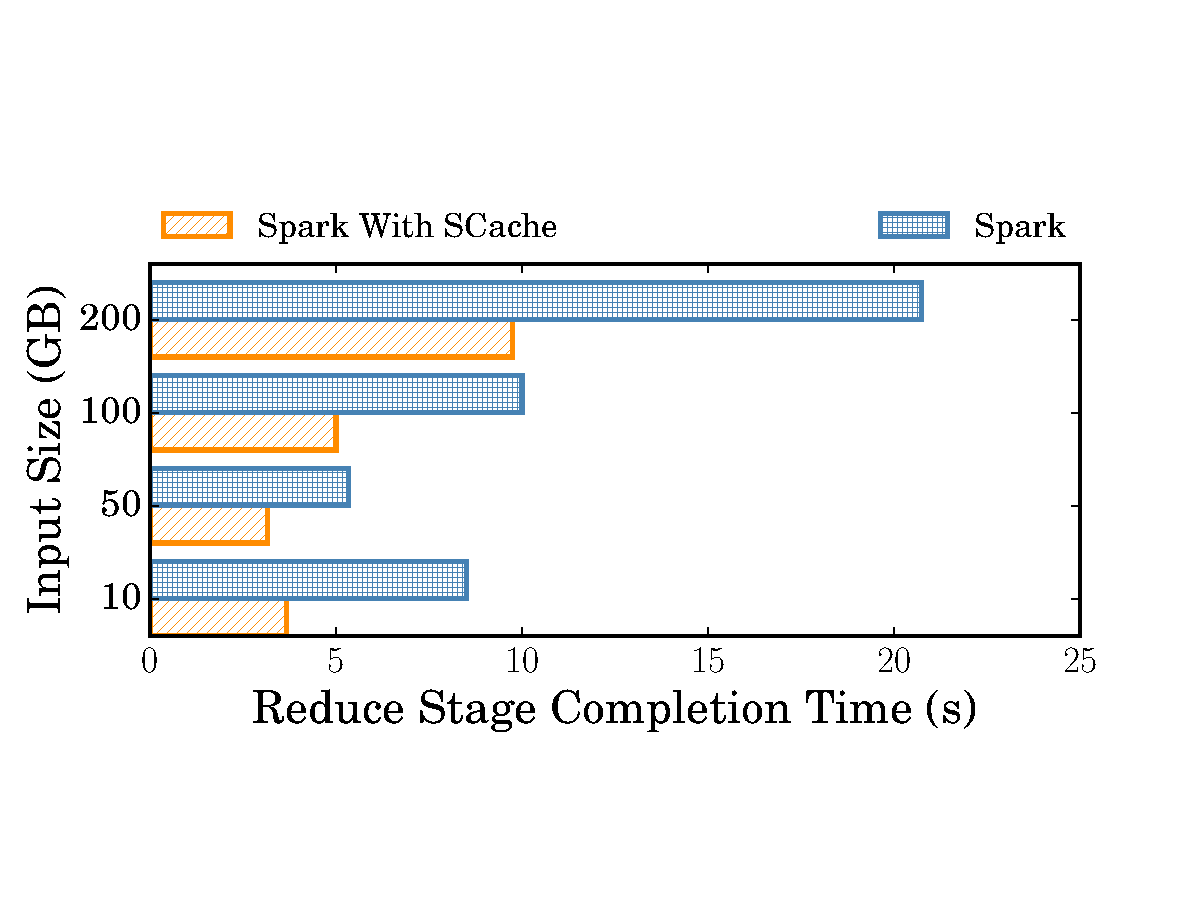
\includegraphics[width=\linewidth]{fig/tera}
				\caption{Reduce Stage of First Shuffle}
				\label{fig:terasort}
			\end{minipage}

			\begin{minipage}{\linewidth}
				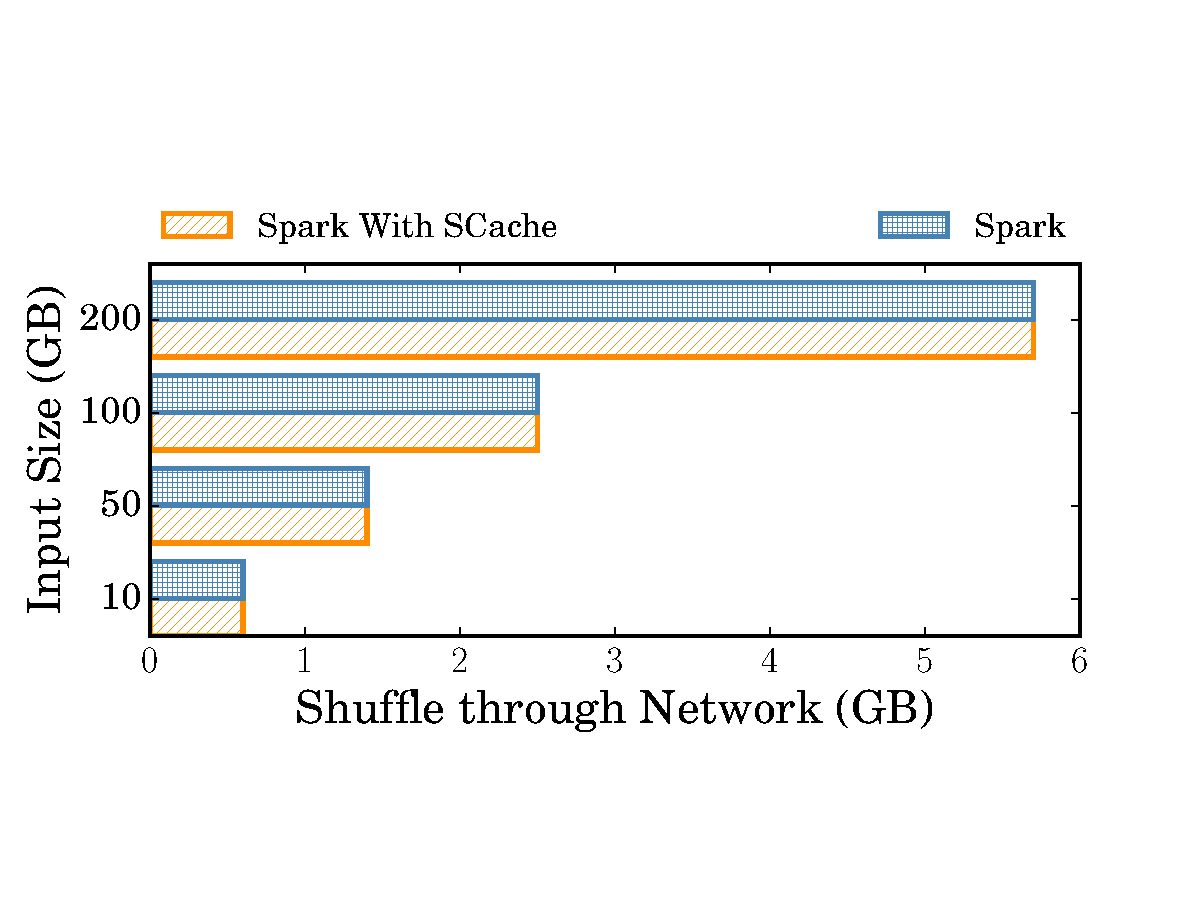
\includegraphics[width=\linewidth]{fig/tera_shuffle}
				\caption{Network Traffic of Second Shuffle}
				\label{fig:terashuffle}
			\end{minipage}
		\end{subfigure}
		\caption{Terasort Evaluation}
	\end{minipage}
\end{figure*}

\subsection{Setup}\label{stepup}
We modified Spark to enable shuffle optimization of SCache as a representative.
The shuffle configuration of Spark is set to the default\footnote{http://spark.apache.org/docs/1.6.2/configuration.html}. 
We run the experiments on a 50-node m4.xlarge cluster on Amazon EC2\footnote{http://aws.amazon.com/ec2/}. 
Each node has 16GB memory and 4 CPUs. The network bandwidth provided by Amazon is insufficient. 
Our evaluations reveal the bandwidth is only about 300 Mbps (see Figure \ref{fig:util}).

\subsection{Simple DAG Analysis}\label{simpledag}
%\subsubsection{Hardware Utilization}
We first run the same single shuffle test shown in Figure \ref{fig:util}. 
For each stage, we run 5 rounds of tasks with different input size. 
As shown in Figure \ref{fig:scache_util}, the hardware utilization is captured from one node during the job. 
Note that since the completion time of whole job is about $50\%$ less than Spark without SCache, the duration of Figure \ref{fig:scache_util} is cut in half as well. 
An overlap among CPU, disk, and network can be easily observed in Figure \ref{fig:scache_util}. 
It is because the decoupling of shuffle prevents the computing resource from being blocked by I/O operations. 
On the one hand, the decoupling of shuffle write helps free the slot earlier, so that it can be re-scheduled to a new map task.
On the other hand, with the help of shuffle pre-fetching, the decoupling of shuffle read significantly decreases the CPU idle time at the beginning of a reduce task.
At the same time, SCache manages the hardware resources to store and transfer shuffle data without interrupting the computing process.
As a result, the utilization and multiplexing of hardware resource are increased, thus improving the performance of Spark. 
% \begin{figure}
% 	%\vspace*{-0.01cm}
% 	\begin{subfigure}{\linewidth}
% 		\centering
% 		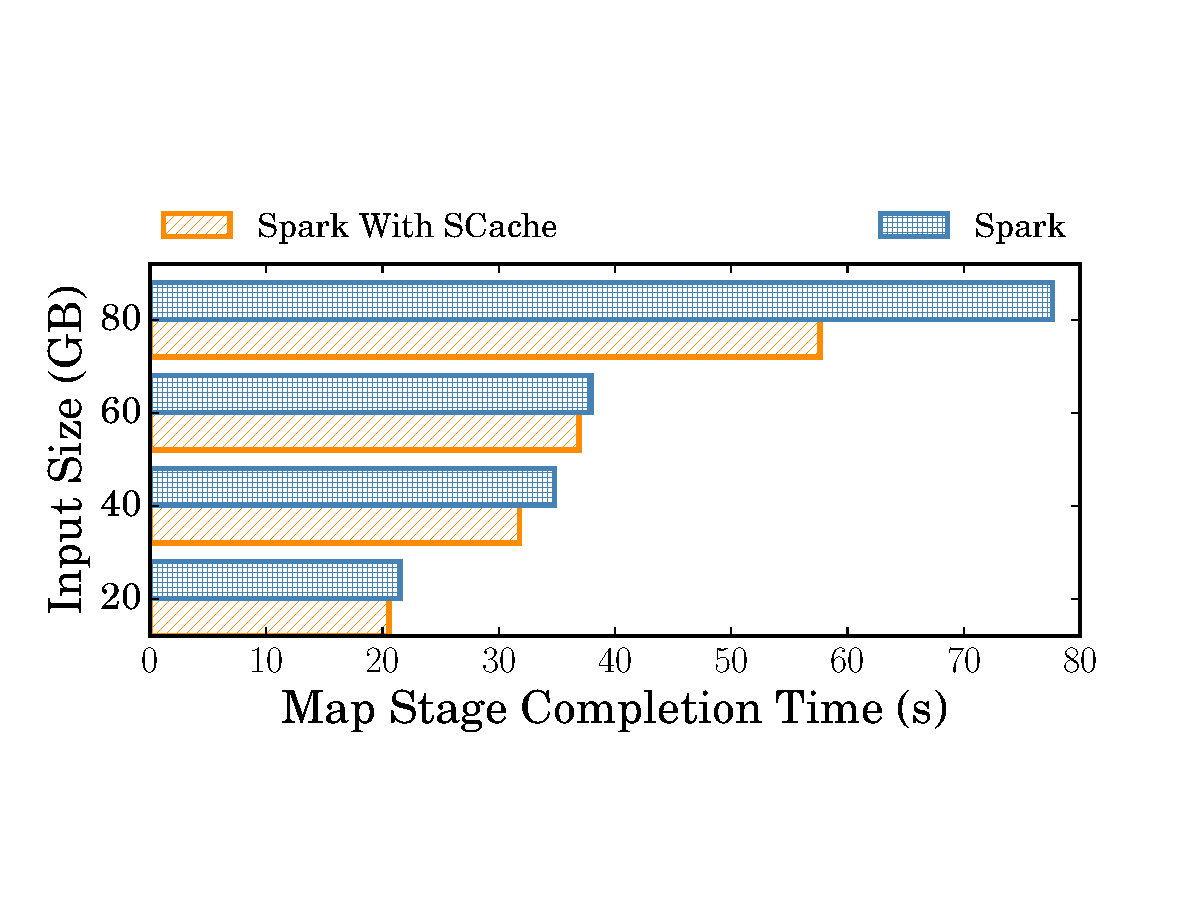
\includegraphics[width=0.6\linewidth]{fig/groupbymapstage}
% 		\caption{Map Stage Completion Time Comparison}
% 		\label{fig:mapstage}
% 	\end{subfigure}
% 	\begin{subfigure}{\linewidth}
% 		\centering
% 		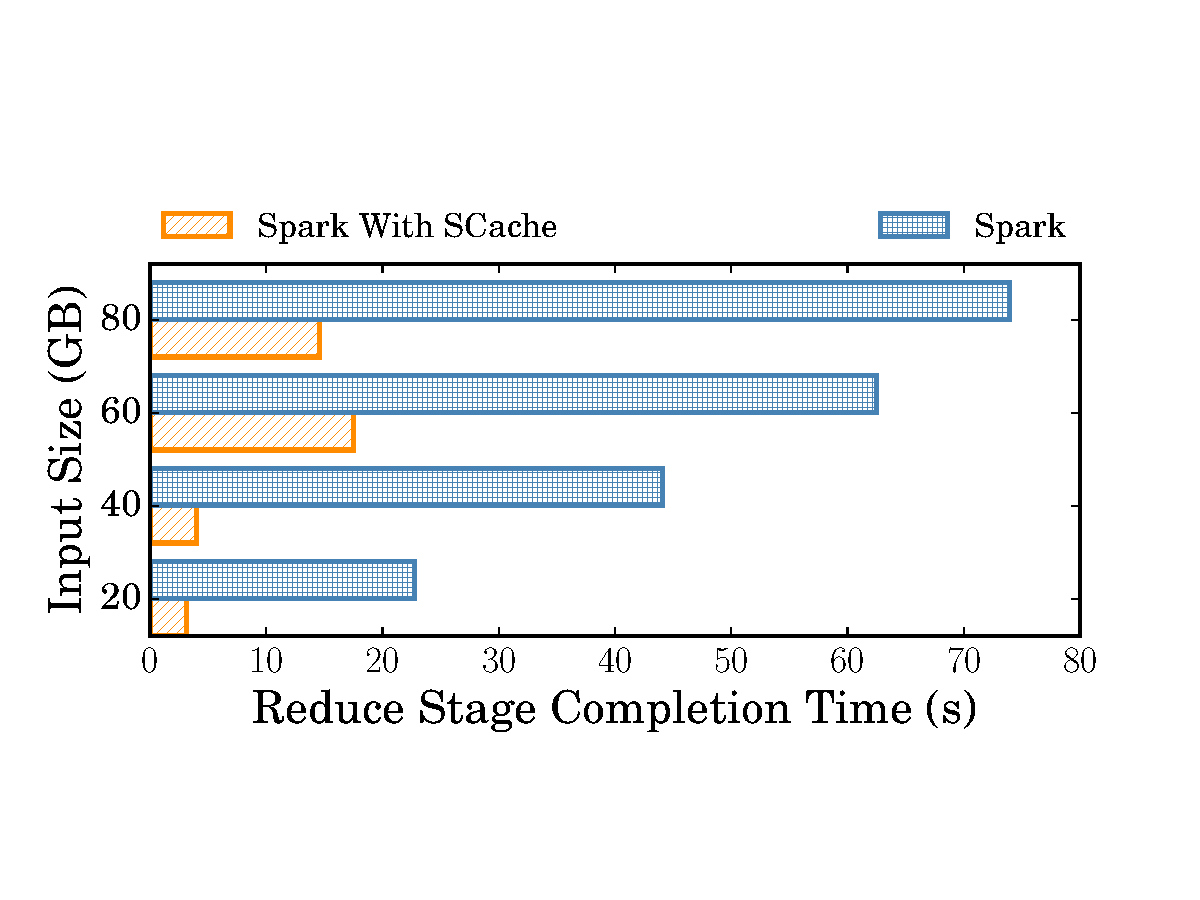
\includegraphics[width=0.6\linewidth]{fig/groupbyreducestage}
% 		\caption{Reduce Stage Completion Time Comparison}
% 		\label{fig:reducestage}
% 	\end{subfigure}
% 	\caption{Stage Completion Time of Single Shuffle Test}
% 	\label{fig:singleshuffle}
% \end{figure}

% \begin{figure}
% 	\begin{subfigure}{\linewidth}
% 		\centering
% 		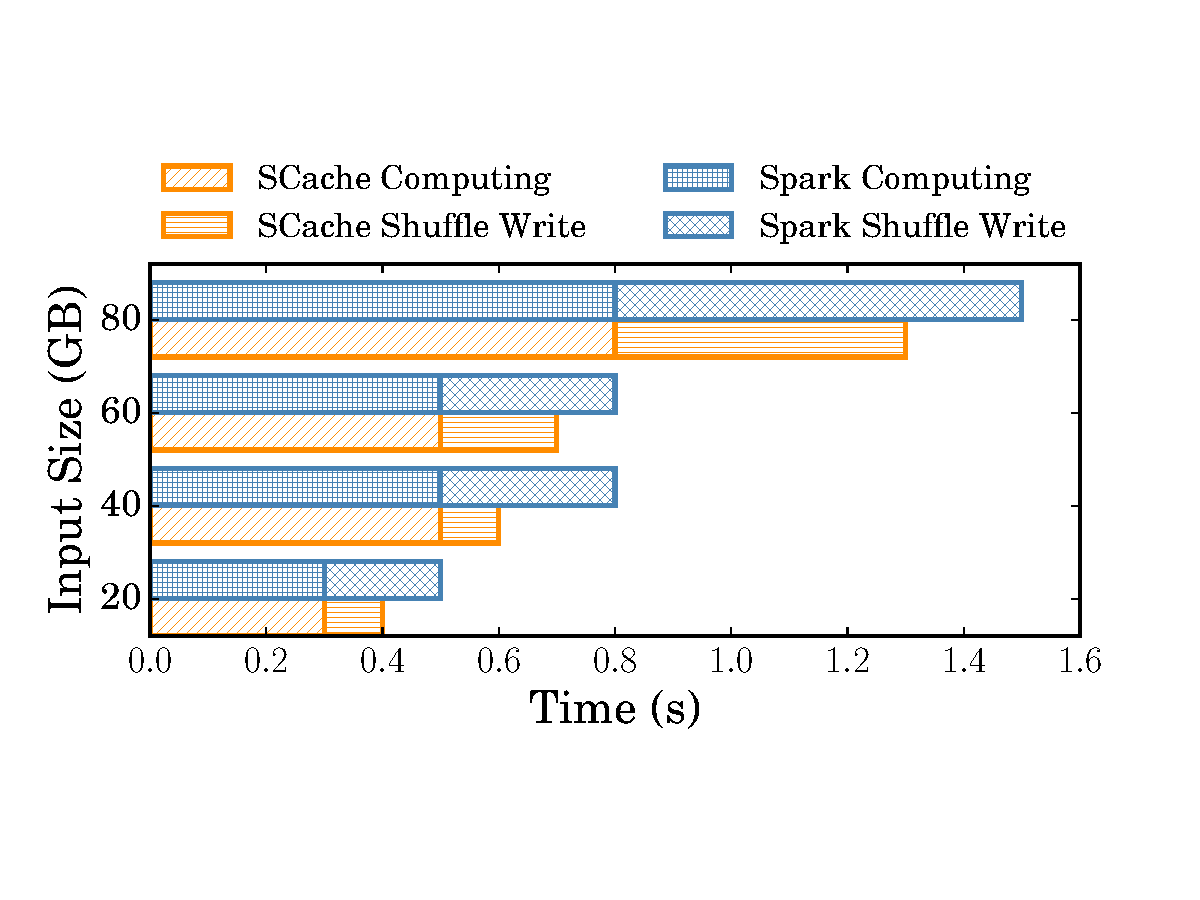
\includegraphics[width=0.6\linewidth]{fig/groupbymaptask}
% 		\caption{Median Task Details in Map Stages}
% 		\label{fig:maptask}
% 	\end{subfigure}
% 	\begin{subfigure}{\linewidth}
% 		\centering
% 		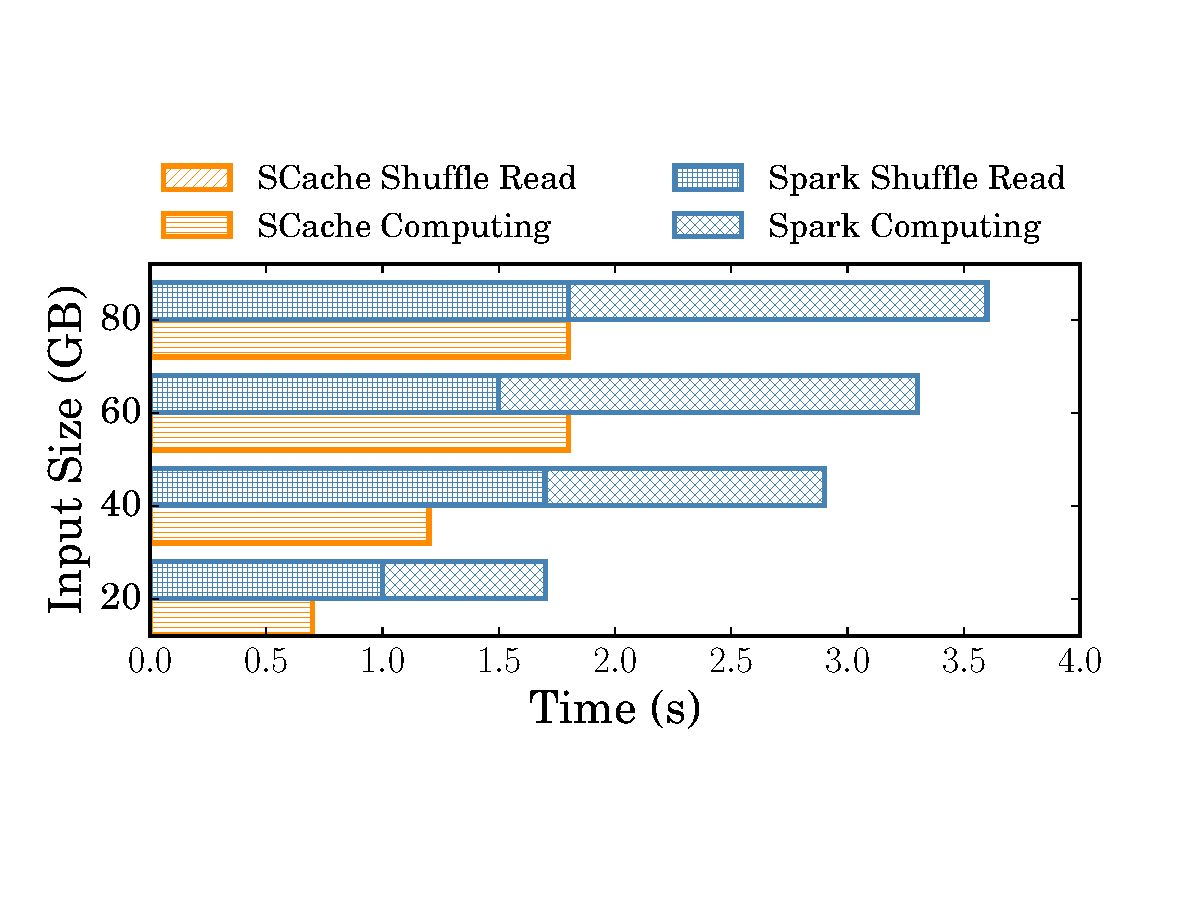
\includegraphics[width=0.6\linewidth]{fig/groupbyreducetask}
% 		\caption{Median Task Details in Reduce Stages}
% 		\label{fig:reducetask}
% 	\end{subfigure}
% 	\caption{Median Task Completion Time of Single Shuffle Test}
% 	\label{fig:singleshuffletask}
% \end{figure}
The performance evaluation in Figure \ref{fig:singleshuffletask} shows the consistent results with our observation of hardware utilization. 
% By running Spark with SCache, the completion time of map stage can be reduced $10\%$ on average. 
% For reduce stage, instead, SCache achieves a ~$75\%$ performance gain in the completion time of the reduce stage.
% A detail analysis into the nutshell of varied overall performance gain on different stages is presented with Figure \ref{fig:singleshuffletask}. 
For each stage, we pick the task that has median completion time. 
In the map task, the disk operations are replaced by the memory copies to decouple the shuffle write. 
It helps eliminate ~40\% of shuffle write time (Figure \ref{fig:maptask}), which leads to a $10\%$ improvement of map stage completion time in Figure \ref{fig:mapstage}. 
Note that the shuffle write time can be observed even with the optimization of SCache. 
The reason is that before moving data out of Spark's JVM, the serialization is inevitable and CPU intensive \cite{makingsense}. 

In the reduce task, most of the shuffle overhead is introduced by network transfer delay. 
By doing shuffle data pre-fetching based on the pre-scheduling results, the explicit network transfer is perfectly overlapped in the map stage. 
With the help of the co-scheduling scheme, SCache guarantees that each reduce task has the benefit of shuffle pre-fetching. 
The in-memory cache of shuffle data further reduce the shuffle read time. 
As a result, the combination of these optimizations decreases ~$100\%$ overhead of the shuffle read in a reduce task (Figure \ref{fig:reducetask}). 
In addition, the heuristic algorithm can achieve a balanced pre-scheduling result, thus providing ~$80\%$ improvement in reduce stage completion time (Figure \ref{fig:reducestage}).

In overall, SCache can help Spark decrease by ~$89\%$ overhead of the whole shuffle process. 

\subsection{Terasort}
We also evaluate Terasort\footnote{https://github.com/ehiggs/spark-terasort}-a recognized shuffle intensive benchmark for distributed system analysis.
Terasort consists of two consecutive shuffles. 
The first shuffle reads the input data and uses a hash partition function for re-partitioning. 
As shown in Figure \ref{fig:terasort}, Spark with SCache runs 2 $\times$ faster during the reduce stage of the first shuffle, which is consistent with the results in Section \ref{simpledag}. 
It further proves the effectiveness of SCache's optimization.

The second shuffle of Terasort partitions the data through a Spark RangePartitioner. 
% As the range bounds set by range partitioner almost match the same pattern of the first shuffle, almost $93\%$ of input data is from one particular map task for each reduce task. So we take the second shuffle as an extreme case to evaluate the scheduling locality for SCache.
In the second shuffle, almost $93\%$ of input data of a reduce task is produced by one particular map task. 
So we take the second shuffle as an extreme case to evaluate the heuristic locality swap of SCache.
In this shuffle, Spark schedules a reduce task to the node that produces most input data. 
By doing this, Spark minimizes the shuffle data through network. 
At the same time, Figure \ref{fig:terashuffle} reveals that SCache produces exactly same network traffic as Spark. 
It implies that the heuristic locality swap of SCache can obtain the best locality while balancing the load. 
\begin{figure}
	\centering
	\begin{minipage}[hb]{\linewidth}
		\begin{subfigure}{\linewidth}
			\begin{minipage}{\linewidth}
				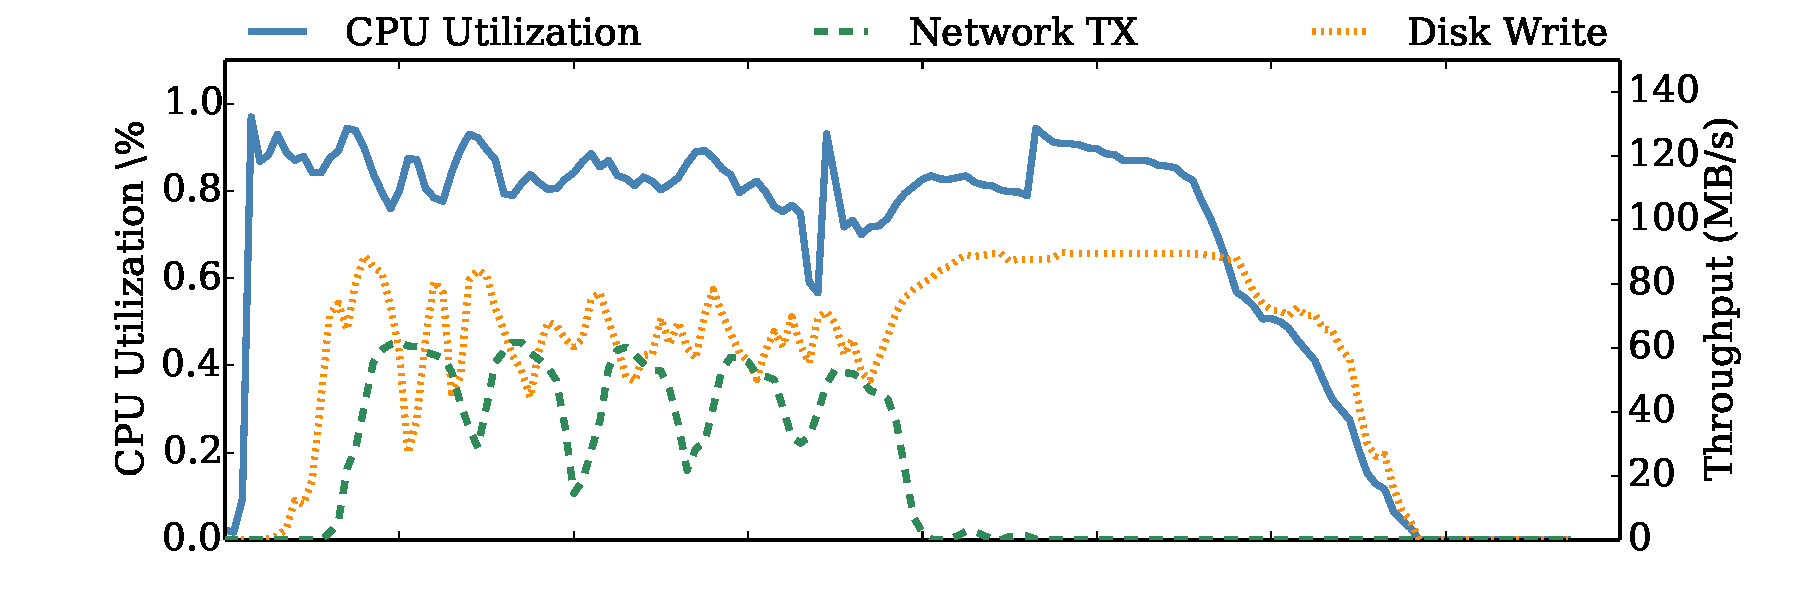
\includegraphics[width=\linewidth]{fig/hadoop_terasort_scache}
				\caption{\color{blue}Hadoop MapReduce With SCache}
				\label{fig:hadoop_terasort_scache}
			\end{minipage}
			\begin{minipage}{\linewidth}
				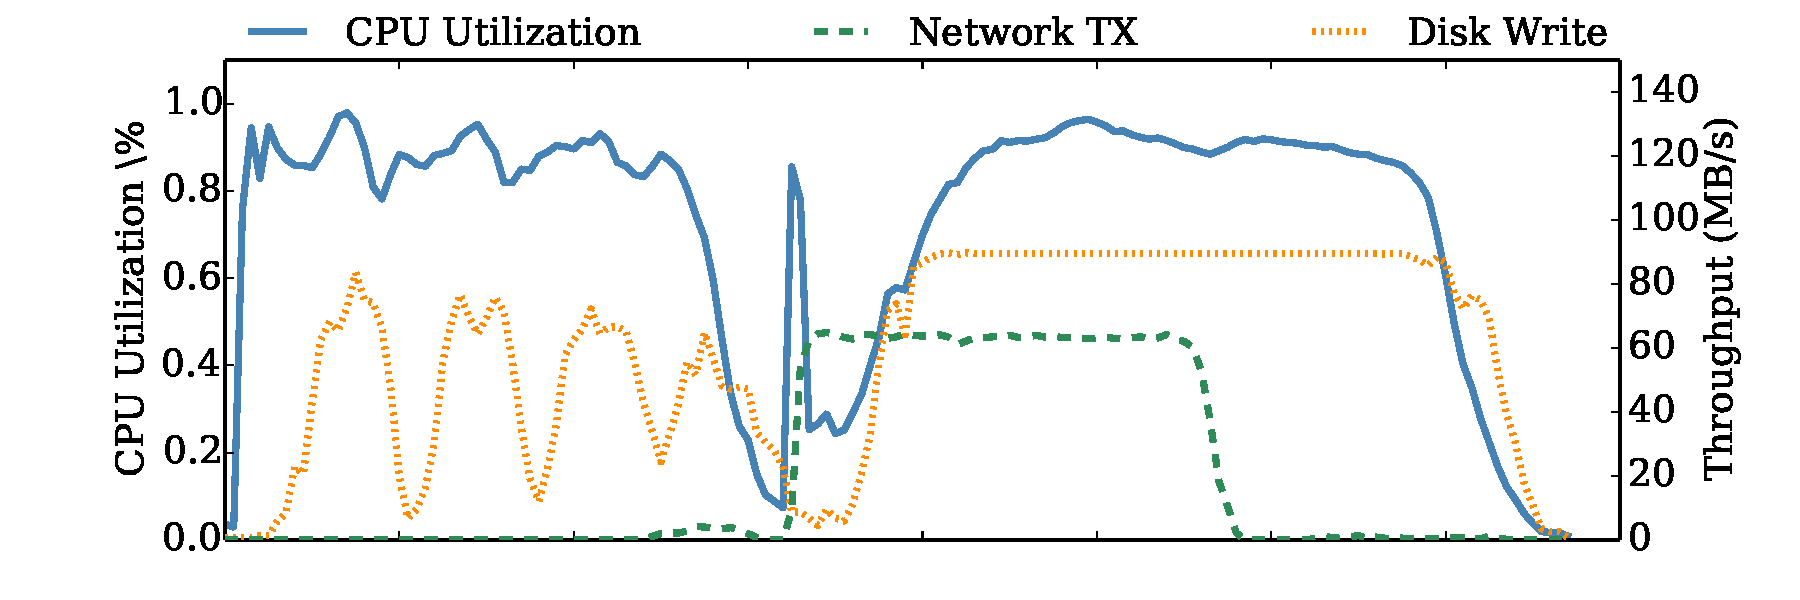
\includegraphics[width=\linewidth]{fig/hadoop_terasort_origin}
				\caption{\color{blue}Hadoop MapReduce Without SCache}
				\label{fig:hadoop_terasort_origin}
			\end{minipage}
		\end{subfigure}
		\caption{\color{blue}CPU utilization and I/O throughput of a node during a Hadoop MapReduce Terasort job}
		\label{fig:hadoop_terasort}
	\end{minipage}
\end{figure}
\begin{figure*}
	\centering
	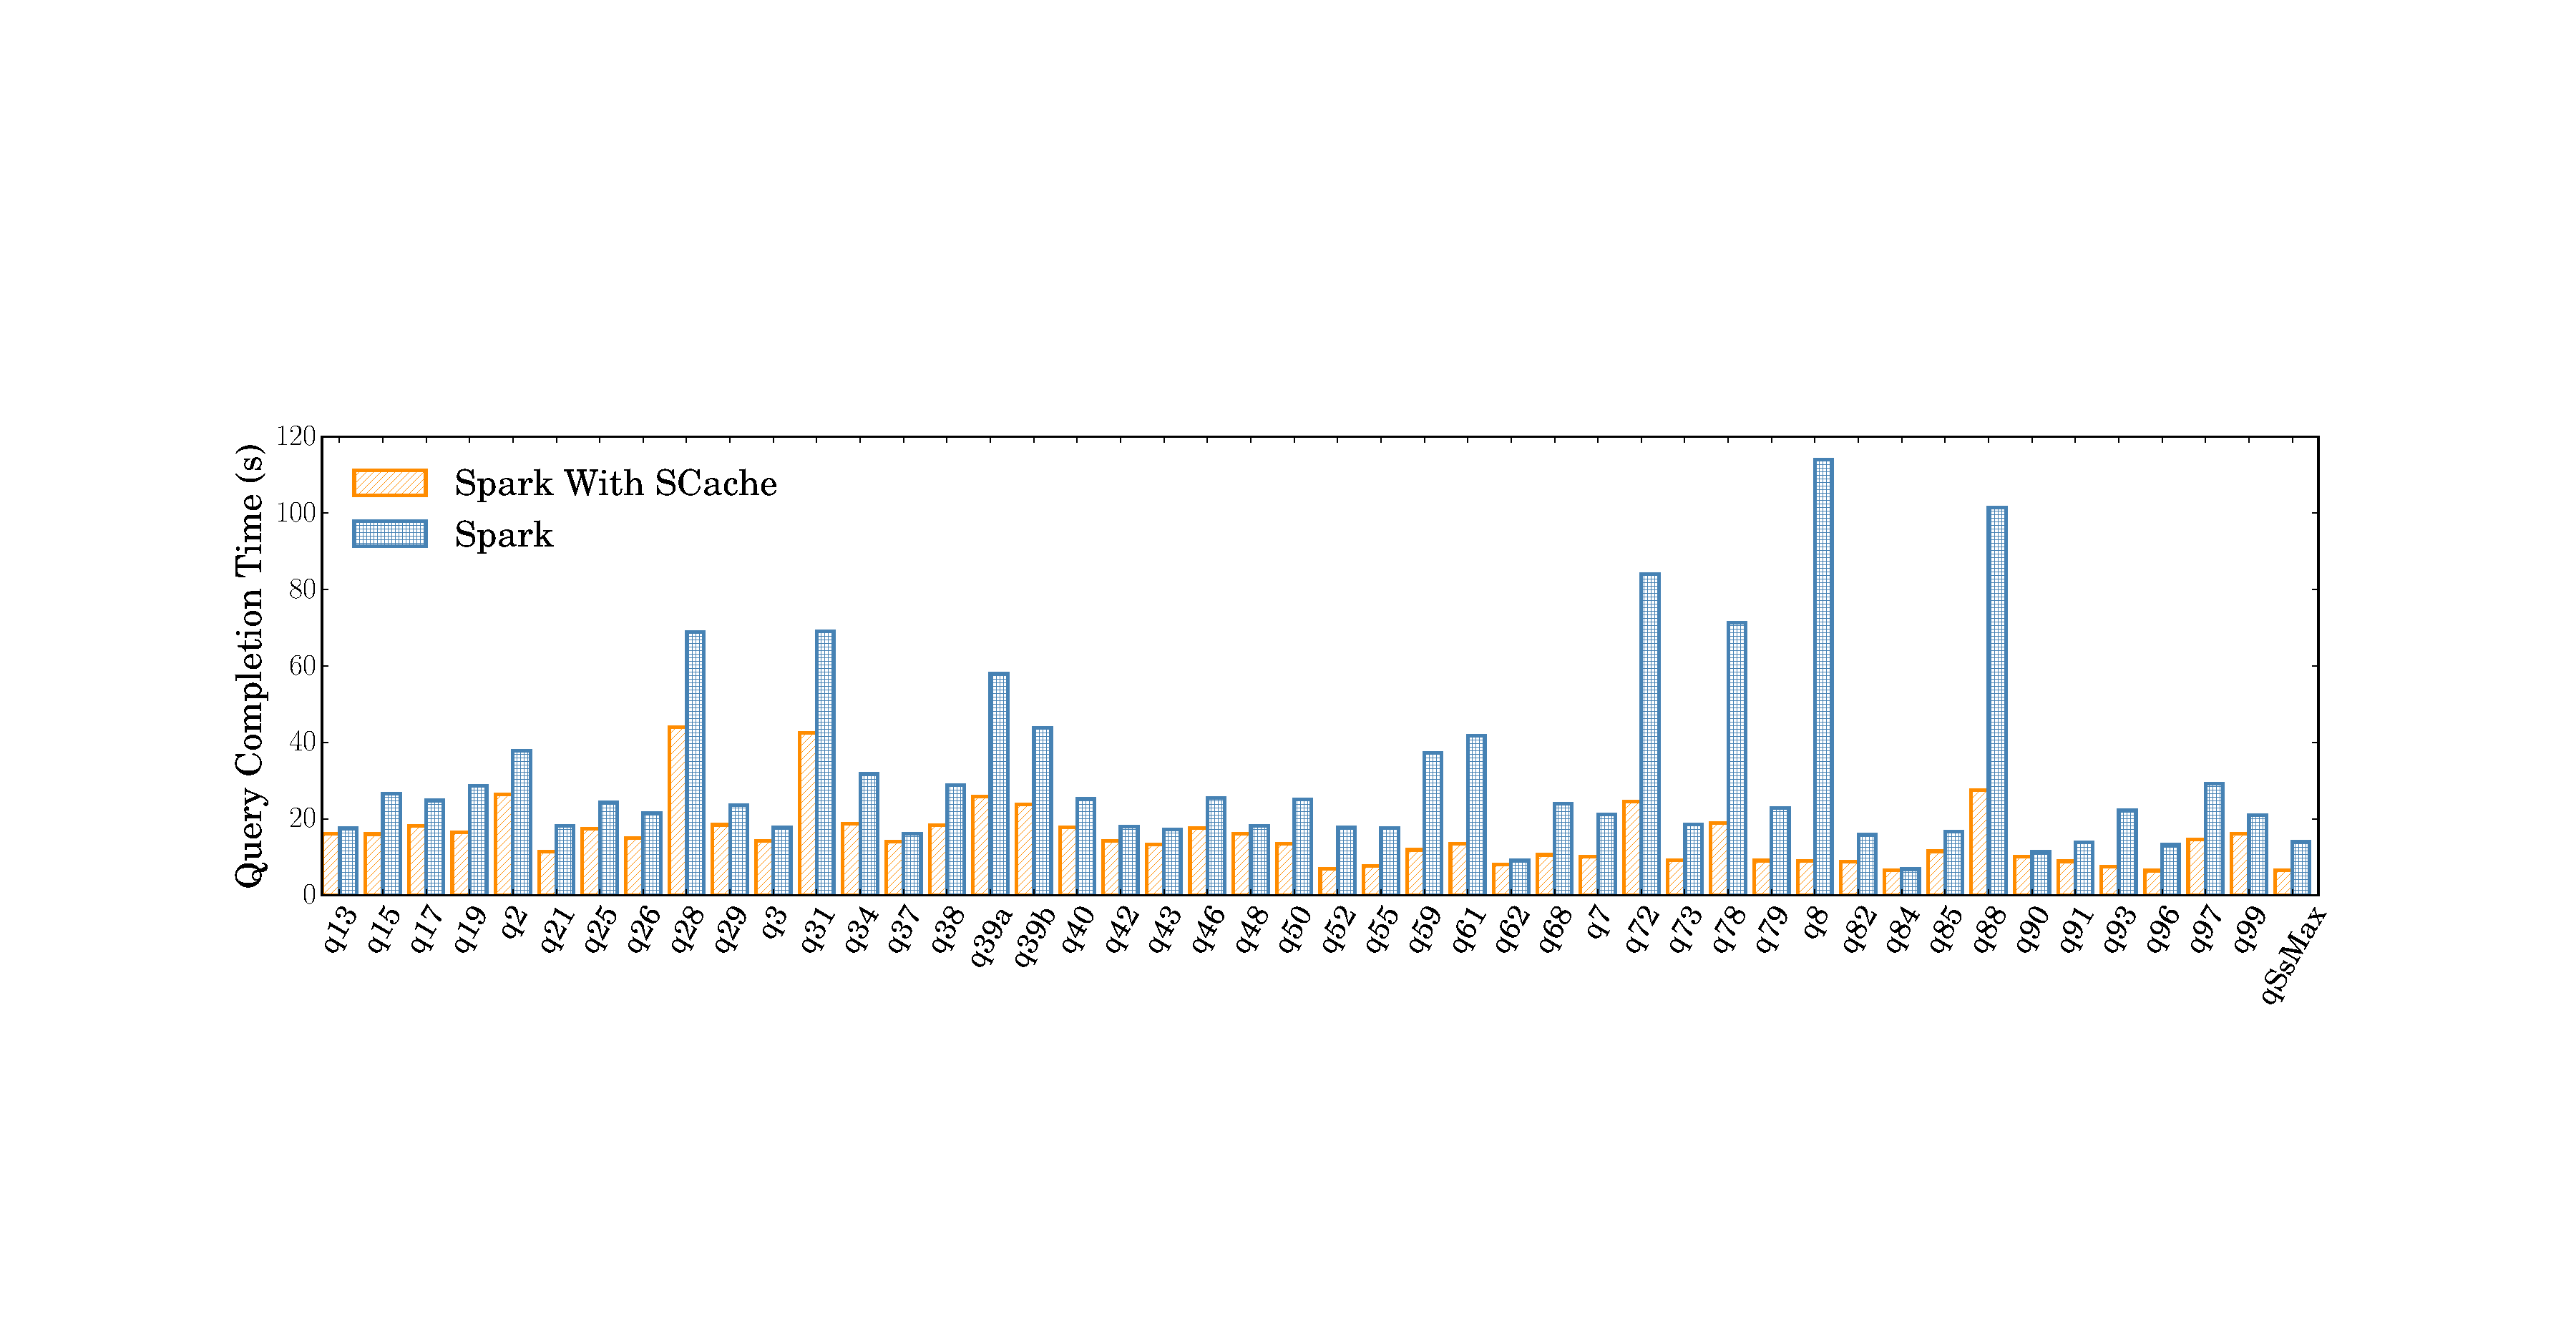
\includegraphics[width=0.85\textwidth]{fig/tpcds}
	\caption{TPC-DS Benchmark Evaluation}
	\label{fig:tpcds}
	\vspace{-1em}
\end{figure*}
\begin{figure}
	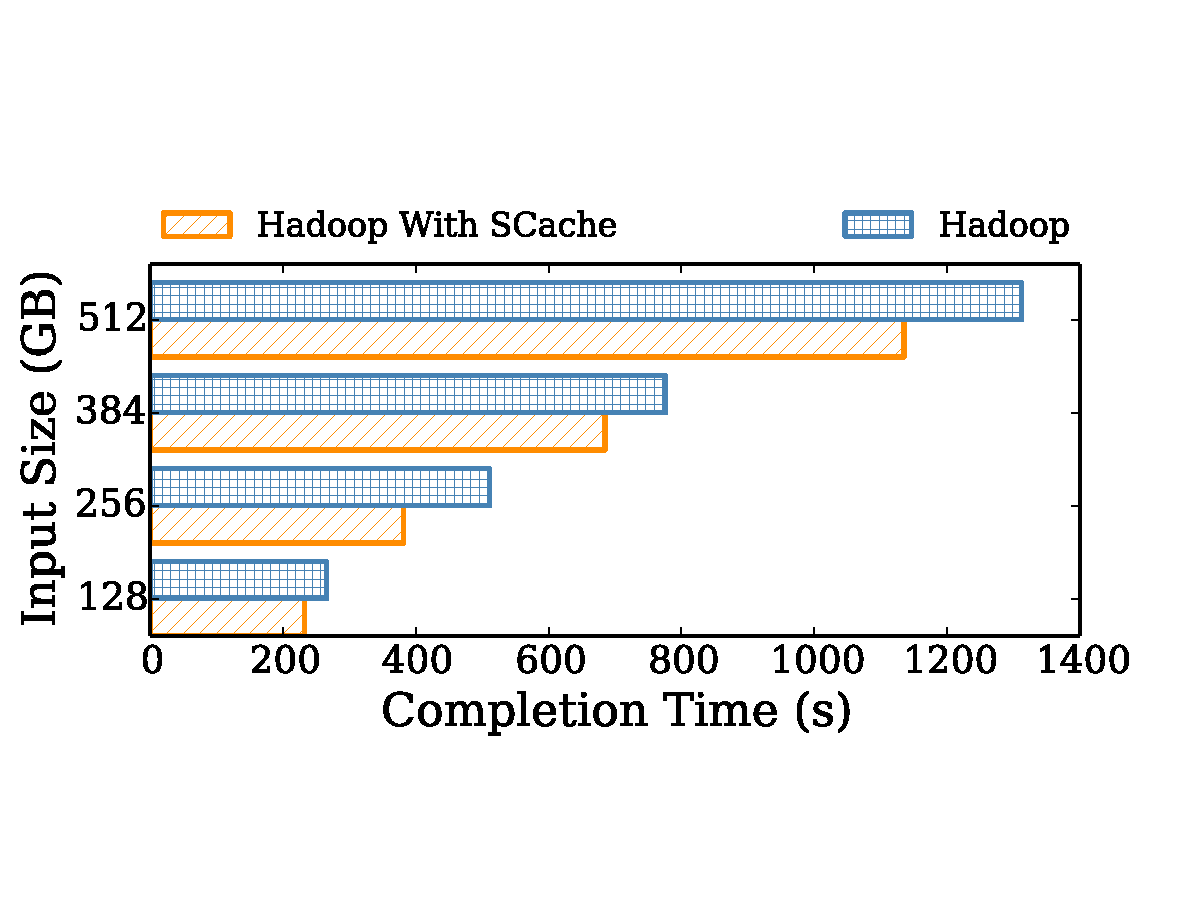
\includegraphics[width=\linewidth]{fig/hadoop_terasort_time}
	\caption{\color{blue}Hadoop MapReduce Terasort completion time}
	\label{fig:hadoop_terasort_time}
\end{figure}


{\color{blue}
\subsection{Hadoop MapReduce with SCache}

To prove SCache compatibility as a cross-framework plug-in, we also implemented SCache on Hadoop MapReduce as the external shuffle service and co-scheduler. Although \textit{pre-scheduling reduce tasks} is not critical for the simple DAG computing such as Hadoop MapReduce, some shuffle-heavy jobs on Hadoop MapReduce can still be optimized by SCache shuffle data management.

Figure \ref{fig:hadoop_terasort} shows the hardware resource utilization of Hadoop MapReduce running Terasort. Both figures have the same proportion of time. Hadoop MapReduce with SCache brings 15\% of total time optimization with 384GB input data size. 
As shown in Figure \ref{fig:hadoop_terasort_origin}, Hadoop MapReduce without SCache writes intermediate data locally in the map phase. The shuffle phase and reduce phase start simultaneously. Because a large amount of shuffle data reaches the network bottleneck, the beginning part of reduce needs to wait for network transfer. This causes the CPU resources to be idle. 
As shown in Figure \ref{fig:hadoop_terasort_scache}, Hadoop MapReduce with SCache start pre-fetching in the map phase. This avoids the reduce phase waiting for the shuffle data. Furthermore, pre-fetching utilizes the idle IO throughput in the map phase. As shown in Figure \ref{fig:hadoop_terasort_time}, after better fine-grained utilization of hardware resources, Hadoop MapReduce with SCache optimize Terasort overall completion time by up to 15\% and an average of 13\% with input data sizes from 128GB to 512GB.
}

\begin{figure}
	\centering
	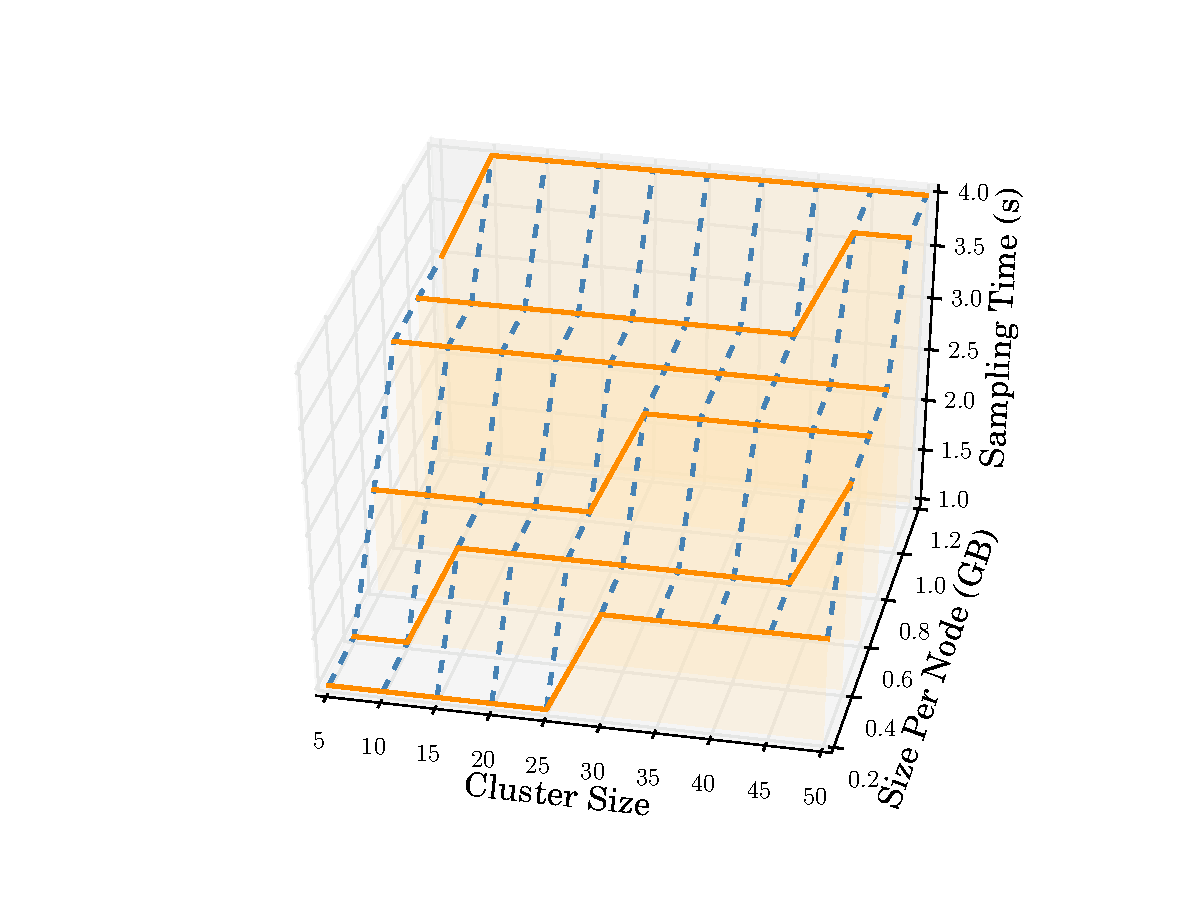
\includegraphics[width=0.6\linewidth]{fig/sampling}
	\caption{Sampling Overhead}
	\label{fig:sampling}
	\vspace{-1em}
\end{figure}

\subsection{Production Workload}
We also evaluate some queries from TPC-DS\footnote{http://www.tpc.org/tpcds/}. 
TPC-DS benchmark is designed for modeling multiple users submitting varied queries (e.g. ad-hoc, interactive OLAP, data mining, etc.). 
TPC-DS contains 99 queries and is considered as the standardized industry benchmark for testing big data systems. 
% We evaluate the performance of Spark with SCache by picking some of the TPC-DS queries with shuffle intensive attribute. 
As shown in Figure \ref{fig:tpcds}, the horizontal axis is query name and the vertical axis is query completion time. 
Note that we skip some queries due to the compatible issues. 
Spark with SCache outperforms the original Spark in almost all tested queries. 
Furthermore, in many queries, Spark with SCache outperforms original Spark by an order of magnitude. 
It is because that those queries contain shuffle-heavy operations such as "groupby", "union", etc.
The overall reduction portion of query time that SCache achieved is 40\% on average. 
Since this evaluation presents the overall job completion time of queries, we believe that our shuffle optimization is promising.
% \begin{figure}
% 	\begin{subfigure}{\linewidth}
% 		\centering
% 		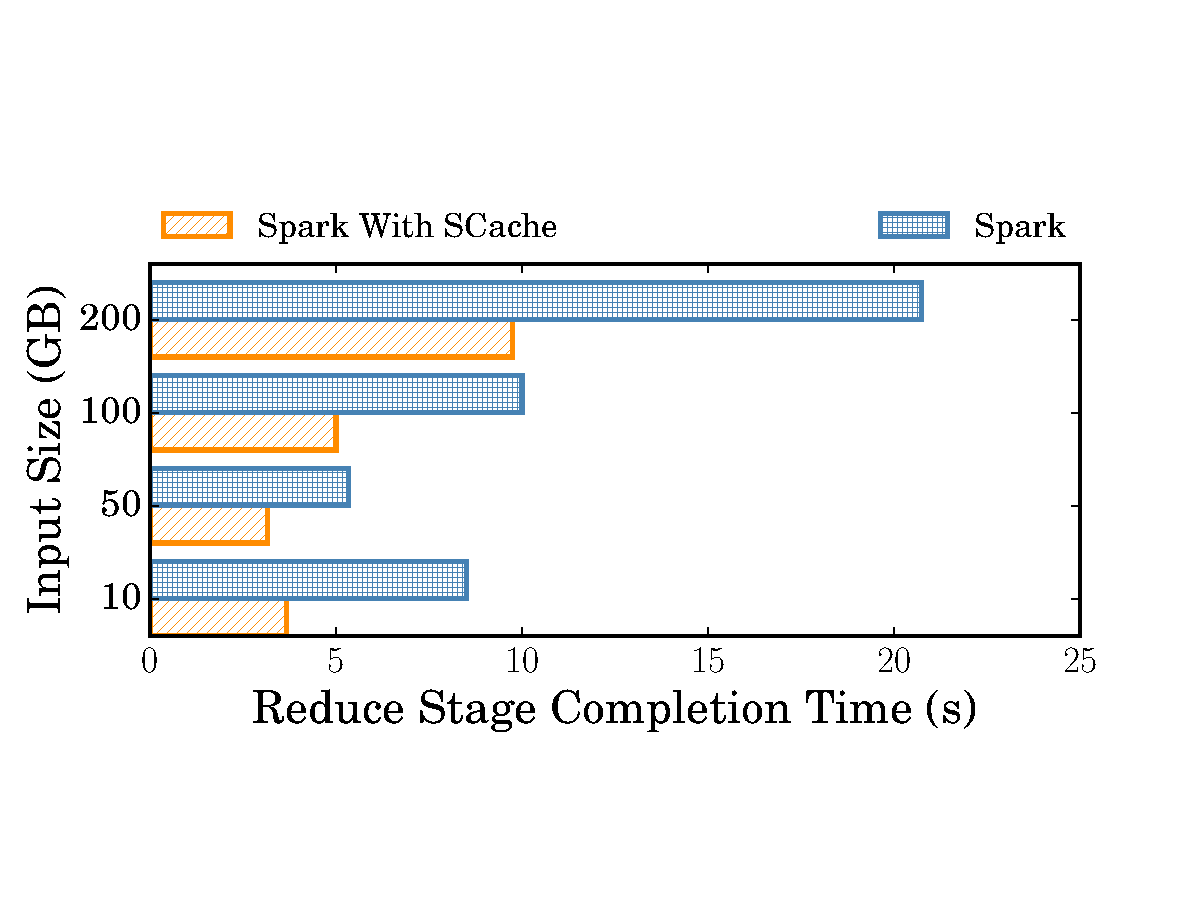
\includegraphics[width=0.6\linewidth]{fig/tera}
% 		\caption{Reduce Stage Completion Time Comparison of First Shuffle}
% 		\label{fig:terasort}
% 	\end{subfigure}
% 	\vspace{0.08cm}
% 	\begin{subfigure}{\linewidth}
% 		\centering
% 		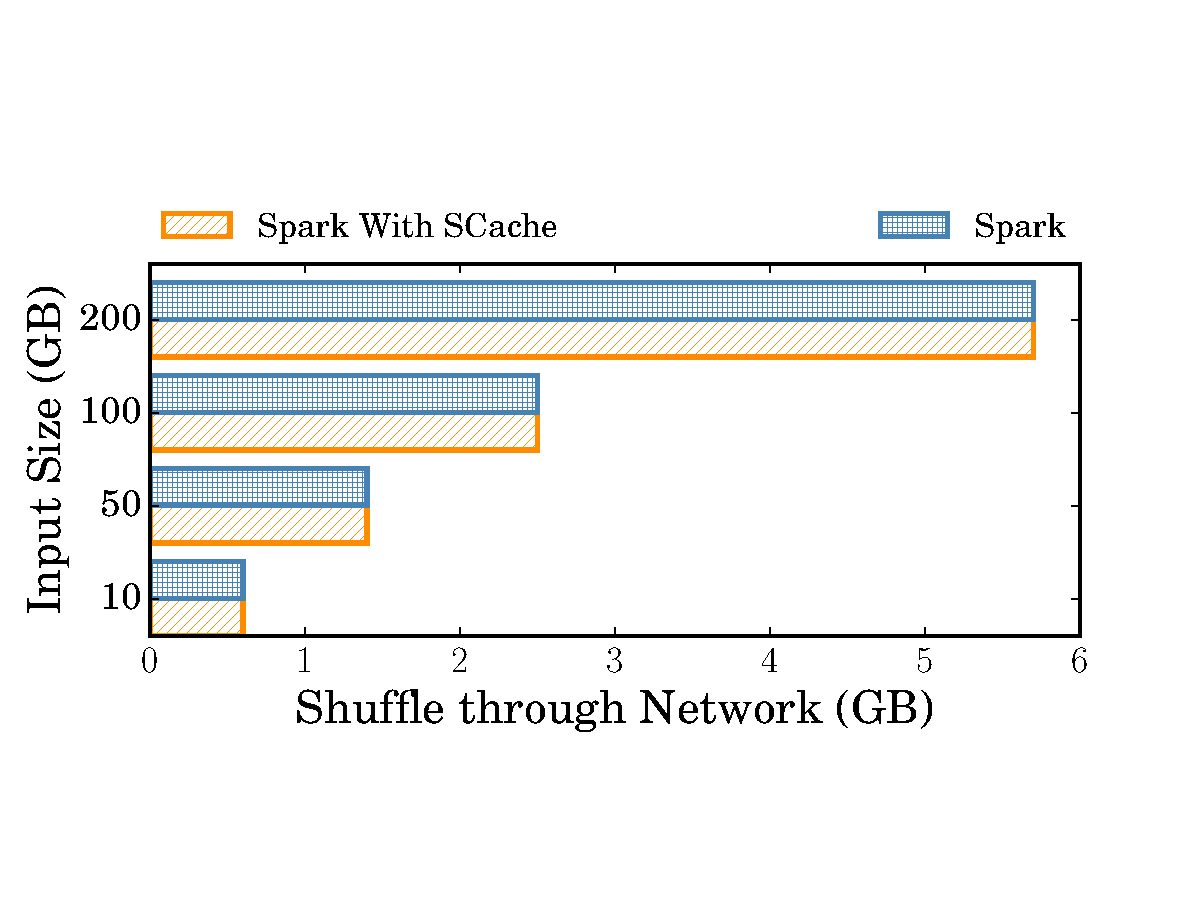
\includegraphics[width=0.6\linewidth]{fig/tera_shuffle}
% 		\caption{Shuffle Data through Network Comparison of Second Shuffle}
% 		\label{fig:terashuffle}
% 	\end{subfigure}
% 	\caption{Terasort Evaluation}
% \end{figure}
\subsection{Overhead of Sampling}
We evaluate the overhead of sampling with different input sizes and numbers of nodes. 
In Figure \ref{fig:sampling}, the overhead of sampling only grows with the increase of input size on each node, but remains relatively stable when the cluster size scales up.
Since the shuffle data is short-lived, write-once, and read-once, the central controller of SCache does not have to collect and manage complex metadata. 
Meanwhile, most of the optimizations such as fetching and storing shuffle data are finished by workers independently. 
So the cost of pre-scheduling algorithm and memory management are unlikely to make the master become the bottleneck of the scalability.
Combined with the sampling overhead evaluation, we believe that SCache is scalable.
